\documentclass[english,10pt,a4paper]{article}
\usepackage[T1]{fontenc}
\usepackage{babel}
\usepackage{fontawesome5}			% To add icons
\usepackage[table]{xcolor}			% To add colors
\usepackage[scale=1]{geometry}      % To manage page margins
\usepackage{graphicx} 				% To add graphics
\usepackage[hidelinks]{hyperref}	% To add link
\usepackage{stix}					% To add block fot skill matrix
\usepackage{fancyhdr}				% To customize header and footer of the page
\usepackage{tikz}
\usepackage{calc}
\usepackage[most]{tcolorbox}
\usepackage{paracol}

\renewcommand{\familydefault}{\sfdefault}

% -------------------------------------------------------------------------------- %
% CV Colors...
% -------------------------------------------------------------------------------- %
\definecolor{CvColor}{RGB}{211,48,93}
\definecolor{CvSidebarBackColor}{RGB}{211,48,93}
\definecolor{CvSidebarTextColor}{RGB}{255,255,255}

% -------------------------------------------------------------------------------- %
% Footer and Header...
% -------------------------------------------------------------------------------- %

\pagestyle{fancy}

% clear existing header/footer entries
\fancyhf{} 
\renewcommand{\headrulewidth}{0pt}

\fancyfoot[L]{\textcolor{CvColor}{\rule[.3\baselineskip]{0.95\textwidth}{1pt}} \quad  \textbf{Page \thepage}}

% -------------------------------------------------------------------------------- %
% Commands...
% -------------------------------------------------------------------------------- %

\newcommand{\skill}[1][3]{%
	\setlength{\unitlength}{1ex}%
	\begin{picture}(1,1.8)
		\linethickness{0.4ex}%
		\textcolor{CvColor!15}{\multiput(0, 0.15)(0, 0.6){3}{\line(1,0){1}}}
		\multiput(0, 0.15)(0, 0.6){#1}{\textcolor{CvColor}{\line(1,0){1}}}
	\end{picture}%
}



% To add level to skill...
\newcommand{\BasicLevel}{{\skill[1]}}
\newcommand{\MediumLevel}{{\skill[2]}}
\newcommand{\MasterLevel}{{\skill[3]}}

% To add level to skill with date...
\newcommand{\BasicLevelDate}[1]{{\skill[1]} {\tiny (#1)}}
\newcommand{\MediumLevelDate}[1]{{\skill[2]} {\tiny (#1)}}

% To add education info in educational section...
\newcommand{\CvEducation}[2]{ {\small \textit{#1}: #2}}

% To add a bullet...
\newcommand{\CvBullet}{\hspace{0.05cm} \textcolor{CvColor}{$\bullet$} \hspace{0.05cm}}
\newcommand{\CvBulletForSidebar}{\hspace{0.05cm}\textcolor{CvSidebarTextColor}{$\bullet$}\hspace{0.05cm}
	}

% Check symbol...
\newcommand{\CvCheck}{\textcolor{CvColor}{\faCheck}}

\newcommand{\CvSection}[2]{\vspace{0.5cm}
	\begin{tcolorbox}[colback=CvSidebarBackColor,boxrule=0pt, top=2.5pt,bottom=2.5pt, arc=0pt,outer arc=0pt]
	{\Large \textcolor{CvSidebarTextColor}{#1 \hspace{2pt} \textbf{#2}}}
	\end{tcolorbox}
	}

% To design 'Time Range'...
\newcommand{\CvTimeRange}[2]{\textcolor{CvColor}{\textsc{#1 - #2}}}

% To design 'Date'...
\newcommand{\CvDate}[1]{\textcolor{CvColor}{{\textsc{#1}}}}

% To desing experience as block...
\newcommand{\FullBlock}{\textcolor{CvColor}{\mdlgblksquare}}
\newcommand{\EmptyBlock}{\textcolor{CvColor}{\square}}

% To customize "itemize" enviroment
\renewcommand{\labelitemi}{$\textcolor{CvColor}{\circ}$}
\renewcommand{\labelitemii}{\textcolor{CvColor}{$\bullet$}}

% -------------------------------------------------------------------------------- %
% Variables.
% -------------------------------------------------------------------------------- %

\def\SidebarHSizeFirstPage{2.5cm}
\def\SidebarHSize{3.95cm}
\def\BodyHSizeFirstPage{9cm}
\def\BodyHSize{12.5cm}

\begin{document}

\columnratio{.31}
\begin{paracol}{2}
	%%%%%%%%%%%%%%%%%%%%%%%%%%%%%%%%%%%%%%%%%%%%%%%%%%
	%%%%%%%%%%%      Contents sidebar      %%%%%%%%%%%
	%%%%%%%%%%%%%%%%%%%%%%%%%%%%%%%%%%%%%%%%%%%%%%%%%%	
	\begin{tcolorbox}[colback=CvSidebarBackColor,height=\textheight,boxrule=0pt, left=0pt,right=0pt,top=0pt,bottom=0pt, arc=0pt,outer arc=0pt]
		\centering
		\begin{tikzpicture}
			\clip (0,0) circle (2cm) node {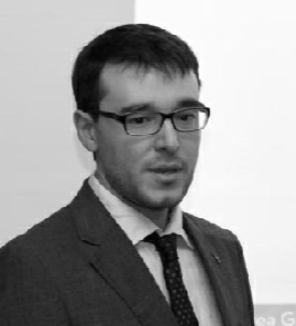
\includegraphics[width=4cm]{./Images/Photo.png}};
			\draw[CvSidebarTextColor, line width=4pt] circle (2cm);
		\end{tikzpicture}
		
		\begin{quotation}
			\textcolor{CvSidebarTextColor}
			{\textsl{Seeking a position that allows me allow me to develop and design  software with ever greater autonomy.\\	
			I would like to work with embedded and real-time systems or develop applications using Linux.\\
			I want to learn and apply DevOps development principles, in
			order to ensure higher quality and maintainability of the
			released software.
			}}
			
		\end{quotation}

		\textcolor{CvSidebarTextColor}{\rule[.5\baselineskip]{0.9\textwidth}{1.5pt}}

		\begin{tabular}{c}
			\\
			\textcolor{CvSidebarTextColor}{\textbf{Place And Date of Birth}} \\
			\textcolor{CvSidebarTextColor}{Frascati, Italy} \\
			\textcolor{CvSidebarTextColor}{27 August 1993 \CvBulletForSidebar \textbf{Age}: 30} \\		
			\\
			\textcolor{CvSidebarTextColor}{\textbf{Address}} \\
		    \textcolor{CvSidebarTextColor}{Viale S. Francesca Saverio Cabrini, 8} \\
	        \textcolor{CvSidebarTextColor}{00077 Monte Compatri (RM), Italy} \\
			\\
			\textcolor{CvSidebarTextColor}{\textbf{Nationality}} \\		
			\textcolor{CvSidebarTextColor}{Italy} \\\\		
			\textcolor{CvSidebarTextColor}{\textbf{Driving Licence}} \\		
			\textcolor{CvSidebarTextColor}{B \CvBulletForSidebar Car Available} \\\\	
		\end{tabular}
	
		\textcolor{CvSidebarTextColor}{\rule[.5\baselineskip]{0.9\textwidth}{1.5pt}}
		
		\begin{tabular}{c}
			\\
			%%%%%%%%%%%%%%%%%%%%%%%%%%%%%%%%%%%%%%%%%%%%%%%%%%
			% Email
			%%%%%%%%%%%%%%%%%%%%%%%%%%%%%%%%%%%%%%%%%%%%%%%%%%
			{\large \textcolor{CvSidebarTextColor}{\faEnvelope}} \\ \href{mailto:andrea.graziani.ing@outlook.com}{\textcolor{CvSidebarTextColor}{\texttt{andrea.graziani.ing@outlook.com}}} \\\\
			
			%%%%%%%%%%%%%%%%%%%%%%%%%%%%%%%%%%%%%%%%%%%%%%%%%%
			% Phone
			%%%%%%%%%%%%%%%%%%%%%%%%%%%%%%%%%%%%%%%%%%%%%%%%%%
			{\large \textcolor{CvSidebarTextColor}{\faPhone}} \\ 
			\textcolor{CvSidebarTextColor}{+(39)~333~78~58~512} \\\\
			
			%%%%%%%%%%%%%%%%%%%%%%%%%%%%%%%%%%%%%%%%%%%%%%%%%%
			% GitHub
			%%%%%%%%%%%%%%%%%%%%%%%%%%%%%%%%%%%%%%%%%%%%%%%%%%
			{\large \textcolor{CvSidebarTextColor}{\textsc{\faGithub}}} \\ \href{https://github.com/AndreaG93}{\textcolor{CvSidebarTextColor}{\texttt{AndreaG93}}} \\\\
			
			%%%%%%%%%%%%%%%%%%%%%%%%%%%%%%%%%%%%%%%%%%%%%%%%%%
			% Linkedin
			%%%%%%%%%%%%%%%%%%%%%%%%%%%%%%%%%%%%%%%%%%%%%%%%%%
			{\large \textcolor{CvSidebarTextColor}{\textsc{\faLinkedin}}} \\ \href{https://it.linkedin.com/in/andrea-graziani-5134b8256}{\textcolor{CvSidebarTextColor}{\texttt{andrea-graziani-5134b8256}}} \\\\
			
		\end{tabular}
		
		\textcolor{CvSidebarTextColor}{\rule[.5\baselineskip]{0.9\textwidth}{1.5pt}}
		
		\begin{tabular}{c}
			\\
		
			%%%%%%%%%%%%%%%%%%%%%%%%%%%%%%%%%%%%%%%%%%%%%%%%%%
			% Available for business travels
			%%%%%%%%%%%%%%%%%%%%%%%%%%%%%%%%%%%%%%%%%%%%%%%%%%
			{\large \textcolor{CvSidebarTextColor}{\faPlaneDeparture}} \\ 
			\textcolor{CvSidebarTextColor}{Available for business travels} \\\\
			
			%%%%%%%%%%%%%%%%%%%%%%%%%%%%%%%%%%%%%%%%%%%%%%%%%%
			% Available for business travels
			%%%%%%%%%%%%%%%%%%%%%%%%%%%%%%%%%%%%%%%%%%%%%%%%%%
			{\large \textcolor{CvSidebarTextColor}{\faGlobeEurope}} \\ 
			\textcolor{CvSidebarTextColor}{Available to relocate abroad} \\
			\textcolor{CvSidebarTextColor}{\textbf{Europe only}}

		\end{tabular}
		
	\end{tcolorbox}
	\switchcolumn  %<--------
	\begin{tcolorbox}[colback=white, height=\textheight,colframe=white, top=0pt,bottom=0pt]
		
		\vspace{1.5cm}
		
		{\Huge \textcolor{CvColor!50}{\textbf{Andrea}} \textcolor{CvColor!80}{\scshape \textbf{Graziani}}} \hfill \\
		\textcolor{CvColor}{\rule[.5\baselineskip]{\textwidth}{2pt}}
		
		
		\hfill {\Large \textcolor{CvColor!60}{\textit{SOFTWARE ENGINEER}}}
		
		\vspace{0.5cm}
		      
		% ================================================================================ %
		% Education
		% ================================================================================ %
		\CvSection{\faGraduationCap}{Education}
		
		% -------------------------------------------------------------------------------- %
		% Master’s Degree
		% -------------------------------------------------------------------------------- %
		\begin{tabular}{p{\SidebarHSizeFirstPage}|p{\BodyHSizeFirstPage}}
			\CvTimeRange{2018}{2022} & \textbf{Master’s Degree}, Computer engineering \\
			& \textsc{Università degli Studi di Roma ``Tor Vergata"} \\
			& \textsc{LM-32 - 2nd level degree in Computer engineering}\\
			& \\
			& \CvEducation{Final degree mark}{\textbf{110/110 cum laude}} \\
			& \CvEducation{Thesis title}{``A QoS-aware broker for multi-provider serverless applications"} \CvBullet \CvEducation{Thesis supervisor}{Valeria Cardellini} \\
			& \CvEducation{Age at graduation}{28} \CvBullet \CvEducation{Graduation date}{23/05/2022}	
		\end{tabular}
		
		\vspace{0.2cm}
		
		% -------------------------------------------------------------------------------- %
		% Bachelor's degree
		% -------------------------------------------------------------------------------- %
		\begin{tabular}{p{\SidebarHSizeFirstPage}|p{\BodyHSizeFirstPage}}
			\CvTimeRange{2012}{2018} & \textbf{Bachelor's degree}, Computer engineering \\
			& \textsc{Università degli Studi di Roma ``Tor Vergata"} \\
			& \textsc{L-8 - 1st level degree in Information technology}\\
			& \\
			& \CvEducation{Final degree mark}{\textbf{102/110}} \\	
			& \CvEducation{Age at graduation}{25} \CvBullet \CvEducation{Graduation date}{26/10/2018}	
		\end{tabular}
		
		\vspace{0.2cm}
		
		% -------------------------------------------------------------------------------- %
		% Diploma
		% -------------------------------------------------------------------------------- %
		\begin{tabular}{p{\SidebarHSizeFirstPage}|p{\BodyHSizeFirstPage}}
			\CvTimeRange{2008}{2012} & \textbf{Italian Secondary School Diploma}, Scientific Certificate \\
			& \textsc{Liceo Scientifico Statale Bruno Touschek} \\	
			& \\
			& \CvEducation{School-leaving examination mark}{\textbf{90/100}} \\
			& \CvEducation{Graduation date}{2012}	
		\end{tabular}
		      
		      % ================================================================================ %
		      % Work Experience
		      % ================================================================================ %
		      \CvSection{\faBriefcase}{Work Experience}
		      
		      \begin{tabular}{p{\SidebarHSizeFirstPage}|p{\BodyHSizeFirstPage}}
		      	\CvTimeRange{June 2022}{Present} & \textbf{Software Engineer}, ALTEN Italia S.p.A. - Rome, Italy \\
		      	& Acted as computer consultant for following companies: 
		      	\begin{itemize}
		      		\item \textbf{ABB S.p.A.} - Rome, Italy \newline
		      		\textbf{(June 2022 - June 2023)} \newline
		      		To develop web applications to perform several task like data management, report extraction, scheduling activities and production monitoring.\newline
		      		\textcolor{CvColor}{\textbf{Activities:}}
		      		\begin{itemize}
		      			\item Acted as software designer, developer, tester and coordinator of the projects.
		      			\item Performed requirements gathering and technical documentation.
		      			\item Handled production deployment, testing and technical support.
		      			\item Started initiatives aimed at improving software development process.
		      			\item Performed bug fixing.
		      		\end{itemize}
		      		\textcolor{CvColor}{\textbf{Results:}}
		      		\begin{itemize}
		      			\item[\CvCheck] Acquired knowledge of several technologies and tools among which ``Entity Framework", Blazor, CSS, C\# and Azure DevOps.
		      			\item[\CvCheck] Improved interpersonal skills.
		      			\item[\CvCheck] Improved ability to work independently.
		      			\item[\CvCheck] Deadlines met with customer satisfaction. 
		      		\end{itemize}
		      	\end{itemize} \\
		      	
		      \end{tabular}
		      
		      
		      
	\end{tcolorbox}
\end{paracol}
\newpage
\newgeometry{left=15mm,right=15mm, top=10mm, bottom=20mm}

\begin{tabular}{p{\SidebarHSize}|p{\BodyHSize}}

& \begin{itemize}
	\item \textbf{GF Machining Solutions S.p.A.} - Meyrin, Switzerland \newline
	\textbf{(June 2023 - September 2023)} \newline
	To develop a web application that allows users to setup and manage laser industrial machines.
	
	\begin{itemize}
		\item Acted as a developer.
		\item Updated technical documentation.
		\item Performed bug fixing.
	\end{itemize}
	
	\textcolor{CvColor}{\textbf{Results:}}
	\begin{itemize}
		\item[\CvCheck] Significanlty improved knowledge about C\#, \texttt{git}, Azure DevOps and Blazor. Acquired a basic knowledge about Scrum. 
		\item[\CvCheck] Slightly improved my confidence in spoken English.
		\item[\CvCheck] Slightly improved my ability to teamwork.
	\end{itemize}
\end{itemize} \\

& \begin{itemize}
	\item \textbf{Telsy Elettronica e Telecomunicazioni S.p.A.} - Rome, Italy \newline
	\textbf{(September 2023 - Present)} \newline
	To develop a desktop application for Microsoft Windows that allows users to exchange data in a secure way.
		
	\begin{itemize}
		\item Acted as a developer.
	\end{itemize}
	
	\textcolor{CvColor}{\textbf{Results:}}
	\begin{itemize}
		\item[\CvCheck] Slighlty improved my knowledge about Windows Presentation Foundation (WPF). Acquired a basic knowledge about Jenkins pipelines.
	\end{itemize}
\end{itemize}

\end{tabular}

		% ================================================================================ %
		% Training
		% ================================================================================ %
		\CvSection{\faBook}{Training}
		
		\begin{tabular}{p{\SidebarHSize}|p{\BodyHSize}}
			\CvDate{September 2022} & \textbf{RabbitMQ usage in event driven architecture} \\
			& \textsc{Training course at ALTEN Italia S.p.A. (Rome, Italy)} \\
		\end{tabular}
		
		% ================================================================================ %
		% Language
		% ================================================================================ %
		\CvSection{\faLanguage}{Language}
		
		\begin{tabular}{p{\SidebarHSize}|p{\BodyHSize}}
			\CvDate{Mother tongue} & Italian \\
			& \\
			
			\CvDate{Foreign language(s)} & \begin{tabular}{c|c|c|c|c}
				\textbf{Language} & \textbf{Listening} & \textbf{Reading} & \textbf{Writing} & \textbf{Speaking} \\
				\hline 
				&&&&\\		
				English & \texttt{B1} & \texttt{B2} & \texttt{B2} & \texttt{B1} \\
			\end{tabular}
		\end{tabular}
		
		\newpage 
		
		% ================================================================================ %
		% Computer Skill
		% ================================================================================ %
		\CvSection{\faLaptop}{Computer Skills}
		
		% -------------------------------------------------------------------------------- 
		% Programming Languages / Markup Languages
		% -------------------------------------------------------------------------------- 
		\begin{tabular}{p{\SidebarHSize}p{\BodyHSize}}		
			\CvDate{Languages} &  \rowcolors{2}{CvColor!15}{white}\begin{tabular}{lcrr}
			
				\centering
				& \textbf{Experience} & \textbf{Experience Years} & \textbf{Last Used} \\
				\hline
				&& \\
				\texttt{C} & $\FullBlock\FullBlock\FullBlock\EmptyBlock\EmptyBlock$ & 2 & 2020 \\
				\texttt{C++} & $\FullBlock\EmptyBlock\EmptyBlock\EmptyBlock\EmptyBlock$ & 0.5 & 2012 \\
				\texttt{C\#} & $\FullBlock\FullBlock\FullBlock\FullBlock\EmptyBlock$ & 1.5 & 2023 \\
				\texttt{Java} & $\FullBlock\FullBlock\FullBlock\EmptyBlock\EmptyBlock$ & 2 & 2020 \\
				\texttt{Go} & $\FullBlock\FullBlock\FullBlock\EmptyBlock\EmptyBlock$ & 1.5 & 2022 \\
				\texttt{Python} & $\FullBlock\FullBlock\FullBlock\EmptyBlock\EmptyBlock$ & 1.5 & 2021 \\
				\texttt{Assembly MIPS} & $\FullBlock\EmptyBlock\EmptyBlock\EmptyBlock\EmptyBlock$ & 0.5 & 2015 \\
				\texttt{Assembly x86} & $\FullBlock\EmptyBlock\EmptyBlock\EmptyBlock\EmptyBlock$ & 0.5 & 2020 \\
				\texttt{HTML} & $\FullBlock\FullBlock\FullBlock\EmptyBlock\EmptyBlock$ & 2 & 2023 \\
				\texttt{CSS} & $\FullBlock\FullBlock\EmptyBlock\EmptyBlock\EmptyBlock$ & 0.5 & 2023 \\
				\LaTeX & $\FullBlock\FullBlock\FullBlock\EmptyBlock\EmptyBlock$ & 4 & 2023 \\\\
			\end{tabular}
		\end{tabular}
		
		\textcolor{CvColor}{\rule[.3\baselineskip]{0.95\textwidth}{1pt}}
		
		\begin{tabular}{p{\SidebarHSize}p{\BodyHSize}} & {\footnotesize For each skill a level is reported according to following scheme} \\
		& {\footnotesize \BasicLevel \hspace{2pt} (Basic) \hspace{4pt} \MediumLevel  \hspace{2pt} (Medium) \hspace{4pt} \MasterLevel \hspace{2pt} (Advanced)}\\ \\\\\end{tabular}
		
		% -------------------------------------------------------------------------------- %
		% Other
		% -------------------------------------------------------------------------------- %
	
		\begin{tabular}{p{\SidebarHSize}p{\BodyHSize}}
			\CvDate{Cloud} & Apache OpenWhisk \BasicLevel \CvBullet AWS EC2 \BasicLevel \CvBullet AWS Lambda  \BasicLevel \CvBullet AWS Step Functions \BasicLevel \CvBullet AWS CloudWatch \BasicLevel \CvBullet SonarQube \BasicLevel \\\\
		\end{tabular}
		
		\begin{tabular}{p{\SidebarHSize}p{\BodyHSize}}
			\CvDate{DevOps and \newline Build automation} & Azure DevOps \BasicLevel \CvBullet JIRA Software \BasicLevel \CvBullet Travis CI \BasicLevel \CvBullet Maven \BasicLevel \CvBullet CMake \BasicLevel \CvBullet Jenkins \BasicLevel \\\\
		\end{tabular}
		
		\begin{tabular}{p{\SidebarHSize}p{\BodyHSize}}
			\CvDate{Databases} & Microsoft SQL Server \MediumLevel \CvBullet PostgreSQL \MediumLevel \CvBullet InfluxDB \BasicLevel \CvBullet Apache Cassandra \BasicLevel \CvBullet Apache Kakfa \BasicLevel \\\\
		\end{tabular}
		
		\begin{tabular}{p{\SidebarHSize}p{\BodyHSize}}
			\CvDate{ORM} & Entity Framework \MediumLevel \CvBullet Hibernate \BasicLevel \\\\
		\end{tabular}
		
		\begin{tabular}{p{\SidebarHSize}p{\BodyHSize}}
			\CvDate{OS} & Microsoft Windows \MediumLevel \CvBullet Kubuntu \MediumLevel \CvBullet KDE Neon \MediumLevel \CvBullet Manjaro \MediumLevel \CvBullet Arch Linux \MediumLevel \\\\
		\end{tabular}
		
		\begin{tabular}{p{\SidebarHSize}p{\BodyHSize}}
			\CvDate{Web Programming} & Blazor \MediumLevel \CvBullet JSP \BasicLevel \\\\
		\end{tabular}
		
		\begin{tabular}{p{\SidebarHSize}p{\BodyHSize}}
			\CvDate{Desktop\newline Programming} & WPF \BasicLevel \CvBullet JavaFX \BasicLevel \\\\
		\end{tabular}
		
		\begin{tabular}{p{\SidebarHSize}p{\BodyHSize}}
			\CvDate{IDE} & Android Studio \BasicLevel \CvBullet CLion \MediumLevel \CvBullet IntelliJ IDEA Community Edition \MediumLevel \CvBullet GoLand \MediumLevel \CvBullet PyCharm Community Edition \MediumLevel \CvBullet Visual Studio \MediumLevel \CvBullet Google Colaboratory (Colab) \BasicLevel \\\\
		\end{tabular}
		
		\begin{tabular}{p{\SidebarHSize}p{\BodyHSize}}
			\CvDate{Testing} & JUnit \BasicLevel \CvBullet MSTest \BasicLevel \CvBullet Moq \BasicLevel \CvBullet Mockito \BasicLevel \\\\
		\end{tabular}
		
		\begin{tabular}{p{\SidebarHSize}p{\BodyHSize}}
			\CvDate{Virtualization} & Hiper-V \BasicLevel \CvBullet VirtualBox \BasicLevel \\\\
		\end{tabular}
		
		\begin{tabular}{p{\SidebarHSize}p{\BodyHSize}}
			\CvDate{Others} & git \MediumLevel \CvBullet docker \BasicLevel \CvBullet Apache ZooKeeper \MediumLevel \CvBullet Valgrind \BasicLevel \CvBullet \texttt{lp\_solve} \BasicLevel \CvBullet  Gurobi \BasicLevel \CvBullet Some deep learning libraries (\texttt{TensorFlow} and \texttt{Keras}) \BasicLevel \CvBullet RabbitMQ \BasicLevel \\
		\end{tabular}
		
	
	
	

	
	
	
	
	
\end{document}










